%% @author Viktor Richter (vrichter)

\chapter{Introduction}\label{chap.introduction}

In this chapter I present the context and overall aim of this thesis.
After a short introduction to the subject, I highlight the problems that can evolve in human interaction with \glspl{artificial agent} in a \gls{smart environment}.
I formulate the overarching goal of this thesis and derive four research questions to approach this goal.
Furthermore, I introduce a \gls{smart environment} which allows this research and in which the relevant experiments take place.
Finally, I give an overview of the structure of this thesis.
% structure

% put yor research in the context of other research
% make readers understand why they should read your report
% give them a framework for understanding it

% 1. Opening context or background. 
\section{Interaction in Smart Environments}

%% overall context
In recent years, \gls{smart home} technologies and \glspl{robot} not only receive a lot of interest in research communities but get increasingly widespread in daily living.
Private homes can be equipped with many sensors and actuators.
Movement detectors, temperature sensors, heating systems, doors, lights, shutters, dishwashers, and more can be connected to automate insignificant and tedious tasks. 
While general purpose social \glspl{robot}, which do chores and serve guests at parties are neither affordable nor available yet, many specialized solutions emerge.
Fully automatic vacuum-cleaners, litter-boxes, pet-feeding machines, and cooking machines perform their task sufficiently good for people to buy and use them in their private homes.
Simultaneously, \Glspl{ipa}---like the Mycroft AI, Amazon Alexa, Microsoft Cortana, Google Assistant, and Apple's Siri---in smart speakers, phones or TVs allow us to retrieve information, or control lights and media playback with simple verbal commands.

%% problem statement
When people interact in a \gls{smart environment}, they do not always interact with an \gls{artificial agent} in the form of a \gls{robot}, virtual assistant, or smart speaker.
They usually interact with other people or do not want to communicate at all (example situations can be seen in \cref{fig:intro}).
\begin{figure}[htbp]
	\centering
	\begin{subfigure}[t]{0.49\textwidth}
	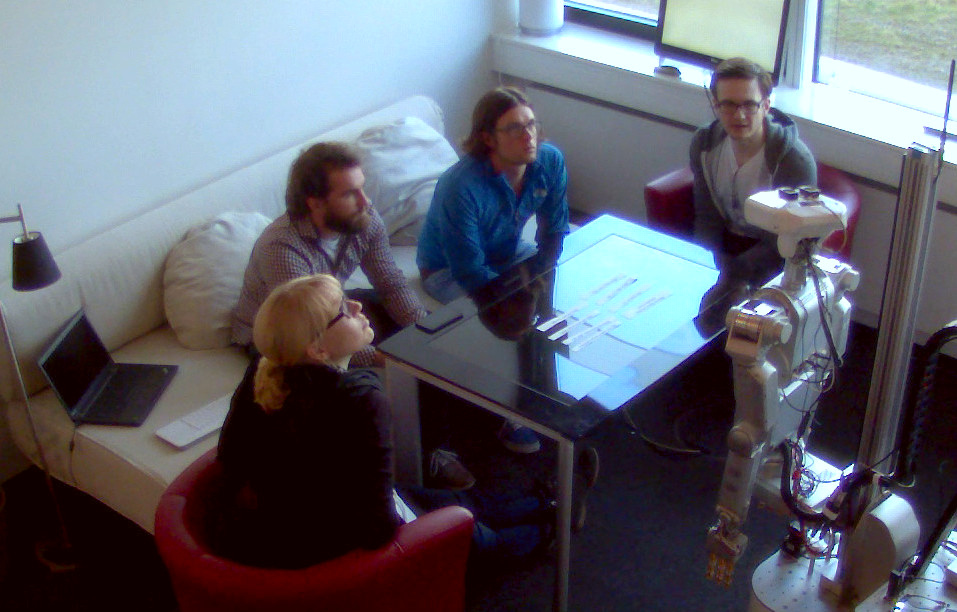
\includegraphics[width=\textwidth]{csra-group-hri}
		\caption{A group interacting with a robot}
		\label{fig:intro.hri}
	\end{subfigure}
	\hfill
	\begin{subfigure}[t]{0.49\textwidth}
	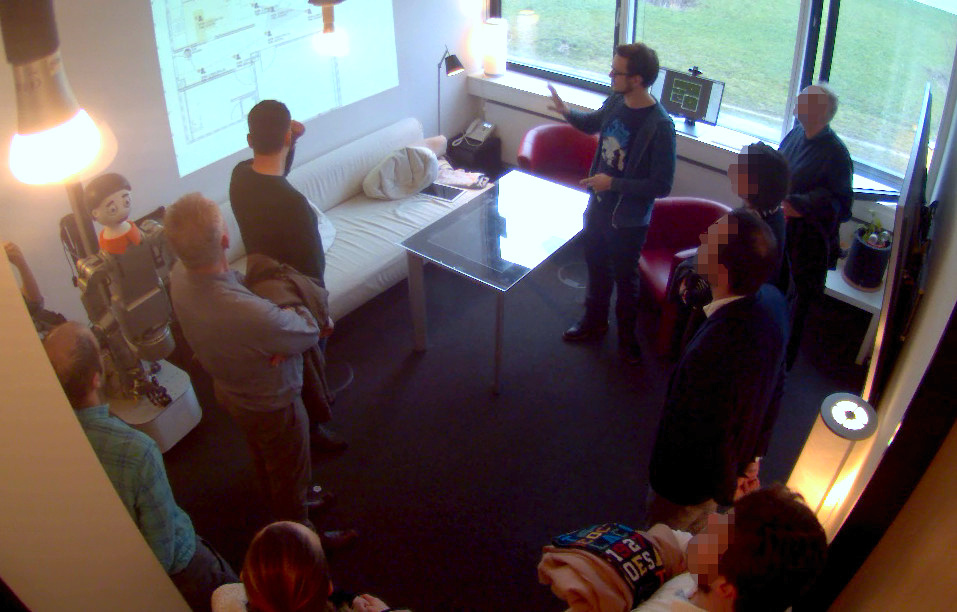
\includegraphics[width=\textwidth]{csra-group-hhi}
		\caption{People interacting with each other}
		\label{fig:intro.hhi}
	\end{subfigure}
	\caption[Interaction with a robot and excluding a robot.]{\label{fig:intro} Two situations as they happen in a \gls{smart environment}. The first picture (\ref{fig:intro.hri}) shows a group of people interacting with a \gls{robot}. The second picture (\ref{fig:intro.hhi}) shows a scene where people speak with each other while the \gls{robot} stands in the background. It is excluded from their interaction.}
\end{figure}
Additionally, there may be multiple groups of conversing people at the same time, each of them trying to interact with an agent or not.
However, gestures and sounds are perceived by everyone in the vicinity, not only by the addressed persons or agents. 
A permanently present agent is required to cope with these problems.
It needs to respond when a person expects it to do so and ignore communication which is not directed at it.
% deeper second problem
Furthermore, according to \gls{tme}~\cite[]{Reeves1996}, people treat systems that show characteristics associated with humans in a human like manner.
This applies to \gls{hci}~\cite[]{Nass1994} and \glspl{ipa}~\cite[]{Lopatovska2018}.
The interaction with such systems elicits social responses in people.
When agents have an embodiment that supports this effect, it gets even stronger.
A \gls{virtual agent} presented by \citewithauthor{Cassell1999} uses \gls{turn taking} signals to enhance the perceived efficiency of the interaction.
According to~\citewithauthor{Mutlu2009}, a \gls{robot} can be used to manipulate the \glspl{conversational role} in an interaction.
The \gls{robot} \emph{Kismet}\footnote{http://www.ai.mit.edu/projects/humanoid-robotics-group/kismet/} can express synthetic emotions to persuade people into nurturing it~\cite{Breazeal1999b}.
Furthermore, in a tutoring scenario with a \gls{robot} presented by~\citewithauthor{Lohan2012}, the human tutors elicit more social communication when the \gls{robot} shows contingent gaze behaviour.
Consequently,~\citefullauthor*{Dautenhahn2005} show that people want \glspl{robot} to communicate in a human-like way and argue for a\newdefgls{robotiquette} to make \gls{hri} acceptable and comfortable to human interaction partners~\cite{Dautenhahn2005,dautenhahn2007socially}.
However, this \gls{robotiquette} does not just require \glspl{robot} to react when addressed.
It poses a set of requirements with increasingly complex challenges from \emph{not standing in the way}, to \emph{showing interest} and \emph{waiting for an adequate moment to talk} to \emph{being considerate and polite}.
To have a chance at fulfilling these requirements, agents need a detailed understanding of human behaviour and expectations towards them.

% 2. A statement of your research question. This is typically a statement of what isn't known or understood or of what is flawed about the research you cited in step 1. It often begins with a but, however, or other word signaling a qualification.
Therefore, the goal of this thesis is to investigate how the sensors of a \gls{smart environment} and contained agents can be used to analyse the \glsatt{conversation} state and expectations of inhabitants.
%To this end I investigate:\todo{it may be better to remove this and bridge directly to RQ}
%\begin{itemize}
%\item How single persons convey the \gls{addressee} of their communication signals.
%\item How an agent, participating in a \gls{conversational group}, can decide if it is addressed or not.
%\item How \glspl{conversational group} with \glspl{artificial agent} can be detected.
%\item How the \glspl{conversational role} of agents can be recognized in multi-centric interactions.
%\end{itemize}
In the following section, I formulate this goal in detail and derive research questions to guide the contributions of this thesis.

% 4. Claim. This answers your research question expressed in step 2.
\section{Research Questions}\label{sec.hypotheses}

People are likely to elicit social behaviours when confronted with a \gls{device} that shows human like characteristics~\cite{Reeves1996}.
However, the level of this effect greatly depends on the persons expectations and the appearance and behaviour of the \gls{artificial agent}~\cite{Hegel2008a}.
Therefore, a varying amount of elicited \glsatt{conversation} cues can be expected for different kinds of agents.
However, as different agents and \glspl{device} have different sensors, they often do not have the sensory means to recognize such cues.
A \gls{smart environment} though, has access to much broader sensing capabilities than its individual agents and the possibility to combine its sensors with the agent's.
Therefore, the overall goal of this dissertation can be stated as follows:
\newcommand{\hypmain}{
	%The perception of a \gls{smart environment} and its agents can be used to monitor human \glsatt{conversation} behaviours to better recognize the \glsatt{conversation} state and expectations of inhabitants towards different kinds of \glspl{artificial agent}.
	Use the perception of a \gls{smart environment} and its agents to recognize the \glsatt{conversation} state and expectations of inhabitants towards different kinds of \glspl{artificial agent}.
	}
\begin{hyp1}
  \label{hyp1}
  \hypmain
\end{hyp1}
To approach this goal, I investigate the following research questions:
\newcommand{\hypaddress}{Which behaviours in \naive{} human interaction with a \gls{smart environment} can be observed  to distinguish which agent is addressed with a deliberate communicational act?}
\begin{hyp2}[Individual Addressing]
	\label{hyp.address}
	\hypaddress
\end{hyp2}
Traditionally, lights and multi-media \glspl{device} are controlled by pushing switches and buttons on the \gls{device} or a remote.
The \gls{addressee} of the touch, thereby, is never ambiguous.
This does not apply to gestures and speech.
In multi-modal interactions the \gls{addressee} of a communicative act is inherently ambiguous and needs to be resolved.
As speech and gestures can be observed by everyone in the vicinity, people need to indicate the \gls{addressee} of their communicative acts.
The same problem arises when people multi-modally control the functionality of a \gls{smart environment}.
Therefore, a set of cues must exist which people use to indicate the \gls{addressee} in such a situation.
\newcommand{\hypmeka}{How can an \gls{artificial agent} visually recognize whether it was addressed by a person within its \gls{conversational group} or not?}
\begin{hyp2}[Addressing in Groups]
  \label{hyp.meka}
  \hypmeka
\end{hyp2}
An interaction of a group of people with a \gls{robot}, naturally does not only contain communication directed towards the latter.
While \glspl{addressee} in verbal interactions are sometimes explicitly stated, this is usually not needed.
To know who is addressed, people utilize their knowledge about the interaction and the behaviour of others.
Therefore, it is necessary for an \gls{artificial agent} to know who is speaking and monitor the \glsatt{conversation} cues of its  interlocutors to be able to distinguish if a statement was addressed at it or not.
%The gaze of the speaker during a statement is an important cue when distinguishing the \gls{addressee} in \gls{hhi} and \gls{hai}~\cite{Vertegaal2001}.   
%A recognition of mouth movements should help verify a \gls{conversational group} member as the groups current speaker. 
\newcommand{\hypfformation}{How can \glspl{focused interaction} of people with \glspl{artificial agent} be automatically recognized in a \gls{smart environment}?}
\begin{hyp2}[Conversational Groups]
	\label{hyp.fformation}
	\hypfformation
\end{hyp2}
Artificial agents are not always part of an interaction.
People dynamically create and change \glspl{conversational group} in which the agent may or may not participate.
Depending on whether the agent is part of an interaction, it can have different options and duties.
On the one hand, it should be open for interactions but not intrusive when nobody wants to interact.
On the other hand, it should actively participate and support the interaction when this is desired.
To be able to fulfil these conflicting requirements, the agent needs to know whether someone (and who) intends to interact with it.
\newcommand{\hyproles}{How to determine \glspl{conversational role} of \glspl{artificial agent} in dynamically changing interactions in a \gls{smart environment}?}
\begin{hyp2}[Conversational Roles]
	\label{hyp.roles}
	\hyproles
\end{hyp2}
Speaker and \gls{addressee} are not the only roles participants of a \gls{conversation} can assume.
Furthermore, these roles do not only exist when one person stops to talk and another begins.
In a \gls{conversation}, all participants assume a role at any given time.
When an \gls{artificial agent} can recognize its \gls{conversational role}, it not only knows when it needs to listen and when to speak.
It can use \glsatt{conversation} cues to influence the distribution of roles in a more informed manner.
Furthermore, it can compare its recognition to its expectations.
It can detect deviations between them, to start repair strategies.

% about the csra
\section{Research Environment}\label{sec.csra}

To specify what a\newdefgls{smart environment} is, I use the definition of~\citefullauthor{Cook2005}:
\blockcquote[p. 3]{Cook2005}{
	A \gls{smart environment} is a small world where all kinds of smart \glspl{device} are continuously working to make inhabitants' lives more comfortable. [\dots] 
	[It] is able to acquire and apply knowledge about an environment and also to adapt to its inhabitants in order to improve their experience in that environment.
}
To be able to investigate the presented research questions, a \gls{smart environment} is needed that not only allows the observation of human interactions with \glspl{device}, but also with \glspl{virtual agent}, and \glspl{robot}.
Furthermore, the execution and recording of corresponding interaction studies should be supported.
The\newdefgls{csra}\footnote{https://www.cit-ec.de/csra}~\cite{Wrede2017} is a laboratory in the \gls{citec}\footnote{https://cit-ec.de} at Bielefeld University which meets these requirements.
If not stated differently, I refer to the \gls{csra} whenever I use the term\newdefgls{apartment}.
It is furnished as a flat with the capabilities of a \gls{smart environment}---so it is a\newdefgls{smart home}---and additionally has the observation and recording capabilities of an interaction laboratory.
Photographs of the \gls{apartment}, its agents and a layout plan be seen in \cref{fig:csra-pics,fig:csra-map-meka}.
\begin{figure}[t]
	\centering
    \def\svgwidth{\textwidth}
    \input{generated/csra-shots.pdf_tex}
	\caption[Virtual agents and scene with robot in the CSRA]{\label{fig:csra-pics} 
	Photographs of the \gls{flobi} agents on the left (\gls{Flobi Entrance} behind the half open door at the top, \gls{Flobi Assistance} from within the kitchen at the bottom). 
	The right picture shows the \gls{apartment} from the outer right end of the living room.
	In this image, two persons are chatting at the table while another is interacting with the \gls{floka} \gls{robot}.
	}
\end{figure}
\begin{figure}[t]
	\centering
    \def\svgwidth{\textwidth}
    \input{generated/LSP-CSRA_Map_2D.pdf_tex}
	\caption[Layout of the CSRA and Floka]{\label{fig:csra-map-meka} 
	On the left, the layout of the \gls{apartment} can be seen.
	The \gls{robot} \gls{floka} is highlighted in green, \gls{Flobi Entrance} in blue, and \gls{Flobi Assistance} in red.
	The right picture shows the \gls{robot} \gls{floka} mounted with it's adapted \gls{flobi} head.
	The sensor head is placed on the floor in front of the \gls{robot}.
	}
\end{figure}
It is a suitable environment to investigate human behaviour and interaction with humans, \glspl{robot}, \glspl{virtual agent} and computers for the following reasons:
\begin{description}
\item[Artificial Agents \& Interactive Appliances:] The \gls{apartment} has multiple interactive \glspl{device}, \glspl{virtual agent} and a \gls{robot} (shown in \cref{fig:csra-pics,fig:csra-map-meka}).
The two virtual \gls{flobi} heads~\cite{Lutkebohle2010,Lier2012}---one in the corridor (\gls{Flobi Entrance}) and one in the kitchen (\gls{Flobi Assistance})---function as the \gls{apartment}'s hosts to welcome and introduce people.
The mobile \gls{robot} \gls{floka}~\cite{Meyer2017} is based on the \emph{MekaBot M1}\footnote{https://robots.ieee.org/robots/m1/}.
It features an anthropomorphic upper body with manipulation capabilities.
Moreover, for its head between the original sensor head and an adapted version of the \gls{flobi} head can be chosen~\cite{Schulz2019}.
Furthermore, the \gls{apartment} contains lights, speakers, screens, door-handles, a pan-tilt beamer, and an interactive plant which can be used to unobtrusively inform people, interact with them or guide their attention.
\item[Variety of Situations:] As a fully integrated smart flat on a university campus, it is used in diverse ways.
Therefore, various kinds of interactions can be observed in it.
In the first place, it constitutes a workspace for the involved staff and students who develop, integrate and test new functionalities and interaction metaphors.
However, demonstrations introduce people to the \gls{apartment} who are not familiar with it and its possibilities.
Meetings and socializing events take place regularly, and finally, it is used to conduct studies.
These can range from human interaction with the \gls{smart environment} to research that is not concerned with \glspl{smart environment} but utilizes the recording and analysis facilities.
\item[Sensors \& Introspection:] The \gls{apartment} features various sensing and recording capabilities.
Four cameras in the corners of the \gls{apartment} provide an overview of the whole situation.
Eight RGBD-Cameras capture the \gls{apartment} from a top-down perspective.
Three Web-cameras provide high resolution video captures from the \glspl{flobi}' viewpoints and for a screen in the living room.
Furthermore, a sensitive floor in the kitchen can detect peoples positions to enrich the \gls{apartment}'s person sensing capabilities.
Microphones capture the global sound and interactions at designated interaction zones in particular.
Movement detectors, sensors for temperature, light, the opening of doors, windows, cupboards, and drawers can be used to follow human physical interaction with the \gls{apartment}.
\item[Availability \& Recording] The \gls{apartment} is operational 24/7 and can automatically record interactions as they occur.
High level information about the \gls{apartment}'s state, the contained agents, and people are available through the~\citesoftware{rsbsoft}.
Compressed video and audio streams are created and accessible via~\citesoftware{gstreamer} and the RTP protocol~\cite{RFC3550}.
All this data can be recorded on demand for studies~\cite{Holthaus2016a} or started and stopped automatically based on usage in a 24/7 operation~\cite{Richter2018}.
\end{description}

% 5. Document structure
\section{Document Overview}

The remaining document is composed as follows.
In the next chapter, I introduce the topic of human \glsatt{conversation} behaviour in focused and \gls{unfocused interaction} from the viewpoint of social sciences.
While at it, I define the relevant terms and models.
Furthermore, I give an overview of the topic of human interaction and \gls{hai} from the viewpoint of computer sciences.
To this end, I additionally establish a taxonomy for the distinction of \glspl{interactive entity} that is applies throughout this thesis.

The central two parts of this thesis, are concerned with the four research questions stated in \cref{sec.hypotheses}.
In \cref{part.addressee}, I investigate human addressing in \glspl{smart environment}.
To this end, I present a study of \naive{} interactions of people with a \gls{smart environment} (\cref{ch.address}).
I examine \cref{hyp.address} by performing an in-depth investigation of the resulting corpus and creating a model for human addressing behaviour towards \glspl{artificial agent} in \glspl{smart environment}.
In \Cref{ch.meka}, I present a mixed \gls{hri} scenario with the anthropomorphic \gls{robot} \gls{floka}.
On this basis, I investigate \Cref{hyp.meka}.
In \cref{part.group}, I aim at a more global understanding of human behaviour in \gls{copresence} with \glspl{artificial agent}.
To this end, I present a scenario and interaction study that allows the analysis of free, dynamically changing \glspl{conversation} of humans with \glspl{artificial agent} (\cref{sec.group.corpus}).
On this basis, I explore \Cref{hyp.fformation} in \cref{ch.fformation} by creating and evaluating a detection framework for mixed human-agent \glspl{conversational group} in a \gls{smart environment}.
In \cref{ch.roles}, I use the models resulting from \cref{ch.meka} and \cref{ch.fformation} to investigate the recognition of \glspl{conversational role} and assess \Cref{hyp.roles}.

In the final part (\cref{part.conclusion}), I summarize the contributions and impact I make with this thesis to research on human interaction with \glspl{smart environment} and \glspl{artificial agent}.
Furthermore, I discuss the limitations of this work, present possibilities for improvement, and give ideas for applications and future research.
